\chapter{Project realization}
\section{Introduction}
This chapter covers the implementation, testing and the deployment processes of
the Benchmarks dashboard project. To deal wit each of these processes, we will
introduce the technologies used and describe the way we used them. In
addition, we will presente the project planning.
\section{Developmnet environment}
\subsection{Devlopment machine characteristics}
The table  TODO presents the characteristics of the developmnet machine we used
during the project implementation.

\begin{center}
  \begin{tabular}{ | p{5cm}  | p{4cm}  | p{2cm} | }
    \hline

    \multicolumn{2}{|c|r|}{Characteristics } & Decription\\
    \hline

\multirow{3}{4em}{Processor} & Type & Intel® Core™ i7-3540M CPU \\ 
\multirow{3}{4em}{Processor} & Type & Intel® Core™ i7-3540M CPU \\ 
\multirow{3}{4em}{Processor} & Type & Intel® Core™ i7-3540M CPU \\ 

     99              & 99        \\ \hline
     99              & 99        \\ \hline

    \hline
  \end{tabular}
\end{center}


\section{Project management}
This section gives an overview of the project management process of the
Benchmarks Dashboard application. At first, we will start by introducing the
project team and then we will describe the tracking process of the different
implementation tasks.
\subsection{Project team}
The table TODO introduces the project team members and their roles.

\begin{center}
  \begin{tabular}{ | p{3cm}  | p{6cm} |}
    \hline

    Scrum role    & Person          \\ \hline

    Product owner & Oussama Elkaceh \\ \hline
    Scrum Master  & Wassel Msehli   \\ \hline
    Team members  & Chaker Benhamed \\ \hline

    \hline
  \end{tabular}
\end{center}

\subsection{Jira tool}
Predictix development teams use Jira for managing the projects. Jira is a
commercial software product developed by Atlassian. It is used for bug tracking,
issue tracking and project management. Jira allow prioritizing, assigning,
tracking, reporting and auditing issues. Indeed, it improves productivity by
cutting down on time wasted on tracking issues and coordination. In fact, it
keeps the team on track and allows the project manager to monitor the progress
on projects. Besides, it improves quality be ensuring that all tasks are
recorded down with all details and followed up until accomplishment. Moreover,
Jira is an extensible platform which means that it offers workflow customization
to match more the business process. TODO(Add link Atlassian, jira software
provider, www.atlassian.com.)


\section{Implementation}
\subsection{Implementation process}
This section describes the whole implementation process step by step TODO
\subsection{Achieved work}
This section is a description of the four sprints and the results we achieved at
the end of each one of them.
\subsection{Sprint 1}
In the first sprint, our goal is to start by automating the benchmark of one of
Predictix's applications, thus we can understand how to generalize for all other
project and solve issue of consistency. The application we worked on is THD-AP.
We started by installing the application locally understand how to build it,
deploy it and how to benchmark it.

After we get acquainted to the benchmark process, we started righting defining
the steps in the benchmark pipeline. 
\subsubsection{Deploying}
To be tested in production-like environment, the
application need to be deployed to the cloud. In order to compare between
benchmarks runs the server in which the application will be deployed need to be
consistent across all the runs The user mustn't have any interaction with the
provisioning of the server nor the deployment of the application. 

$\bullet$ \textbf{Provisioning}: Since Predictix application are
memory-intensive, we chose to deploy them in a r3.4xlarge EC2 instances from
Amazon AWS. This type of instances offer lower price of GiB of RAM. r3.4xlarge
has 122 GB of RAM with 16 cores CPU and 320 GB of SSD Storage.

$\bullet$ \textbf{Installing}:After provisioning the server. We need to deploy
the application to that server. The closure of the application will be already
built in Hydra. We will be using an existent nix configuration to install the
application. It uses a systemd service called \emph{install-app}. This service
will start the database, the web-server, install workspaces and it will make
sure that the application is up and running.

For starting the deployment we use NixOps Dashboard, it will take
some arguments like the type of the instance TODO.

\subsubsection{Load data}
Loading data is project specific, each application need to provide the steps to
download data from S3, extract them and run the necessary workflows to load the
data into the database. Those steps will be written in a script called
\emph{load-perf-data.sh} by the application developers, the script will be ran as
soon as the application in installed. It will be expected to be at the script
directory within the application root directory. The figure
\hyperref[fig:load-perf-data]{\ref{fig:load-perf-data}} shows the definition of
the systemd service \emph{load-perf-data.sh}. And the figure
\hyperref[fig:load-perf-data-running]{\ref{fig:load-perf-data-running}} Shows
the log of systemd service and how the service is invoked automatically.
\begin{figure}[h]
  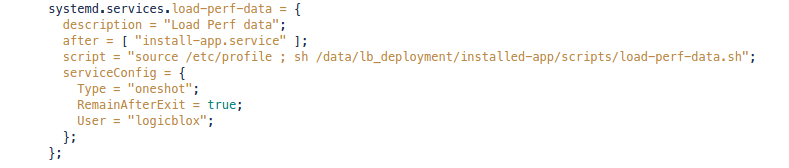
\includegraphics[width=14cm]{load-perf-data}
\caption{Load perf data nix expression}
\label{fig:load-perf-data}
\end{figure}

\begin{figure}[h]
  \centerline{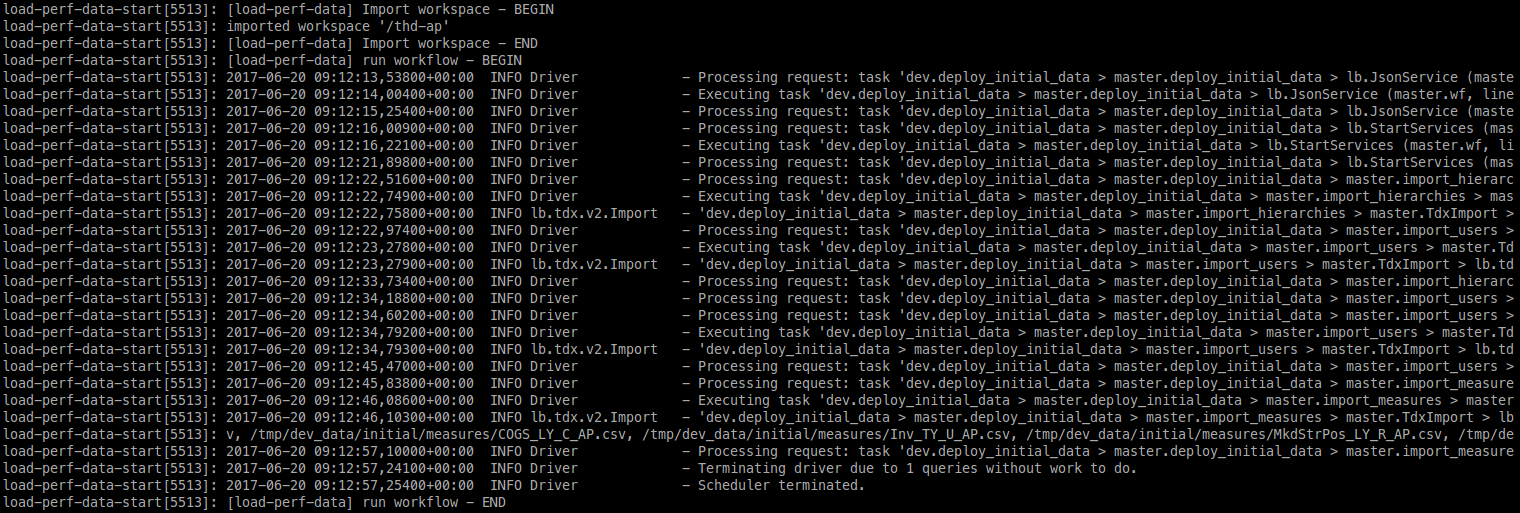
\includegraphics[width=14cm]{load-perf-data-running}}
\caption{load-perf-data log}
\label{fig:load-perf-data-running}
\end{figure}

\subsubsection{Running tests}
For running tests we use a generic script called \emph{run-perf}. This script will
define the instructions for running the tests, collect the logs, generate the
report and upload it to S3. The figure
\hyperref[fig:perf-runner]{\ref{fig:perf-runner}} shows the definition of
the systemd service \emph{perf-runner} responsible for running the script, it
will be launched as soon as the data is loaded with the \emph{load-perf-data}
service.
\begin{figure}[h]
  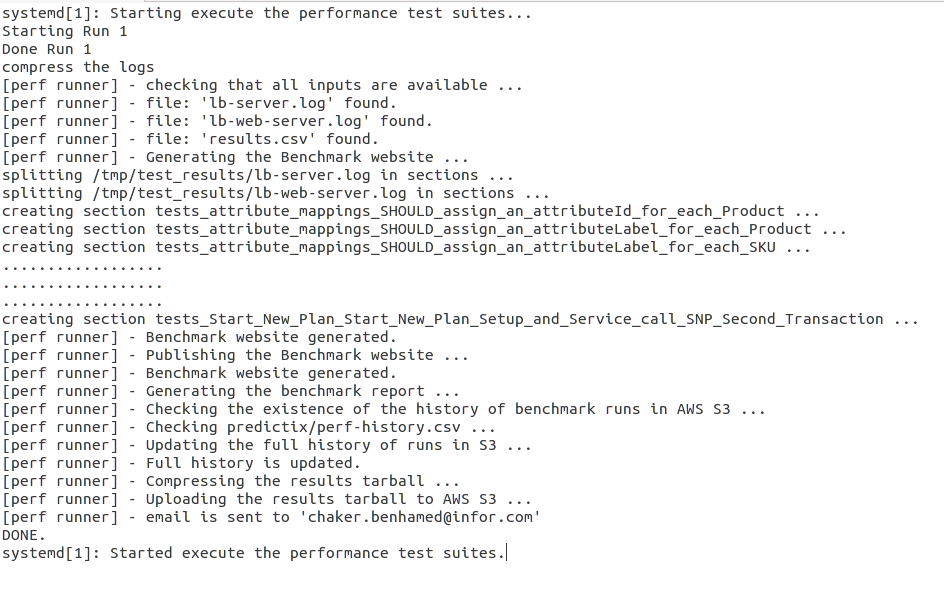
\includegraphics[width=14cm]{perf-runner}
\caption{Load perf data nix expression}
\label{fig:perf-runner}
\end{figure}


\section{Deployment}
Hydra is a Nix-based continuous build system that constantly checks out code
sources of software projects from version management systems such as Mercurial,
to build, test and release them. The build tasks are described using Nix
expressions. This allows a Hydra build task to specify all the dependencies
needed to build or test a project.

In fact, the code of our application is, currently and constantly pushed in a
repository in BitBucket, which is a web-based hosting service for projects that
use either the Mercurial or Git revision control systems, such as GitHub. In
order to have our application ready to be deployed, we added a file called
default.nix to our project, that actually defines our project’s nix-expressions.
Afterwards, we created a project under Hydra, that we called \emph{Benchmarks
  Dashboard}. Thus, the \emph{Benchmarks Dashboard} project on Hydra, will be
pulling our code from our BitBucket repository along with the default.nix file
in order to perform the automated build and unit-tests.

The following are some screen shots about our Hydra project build. The figure
\hyperref[fig:hydra_configuration]{\ref{fig:hydra_configuration}}
represents the configuration for our project. We can notice that the links to the
different project's dependencies are defined, such as our source code and the
nixpkgs repository which contains the definitions for all packages available through
the nix package manager.

\begin{figure}[h]
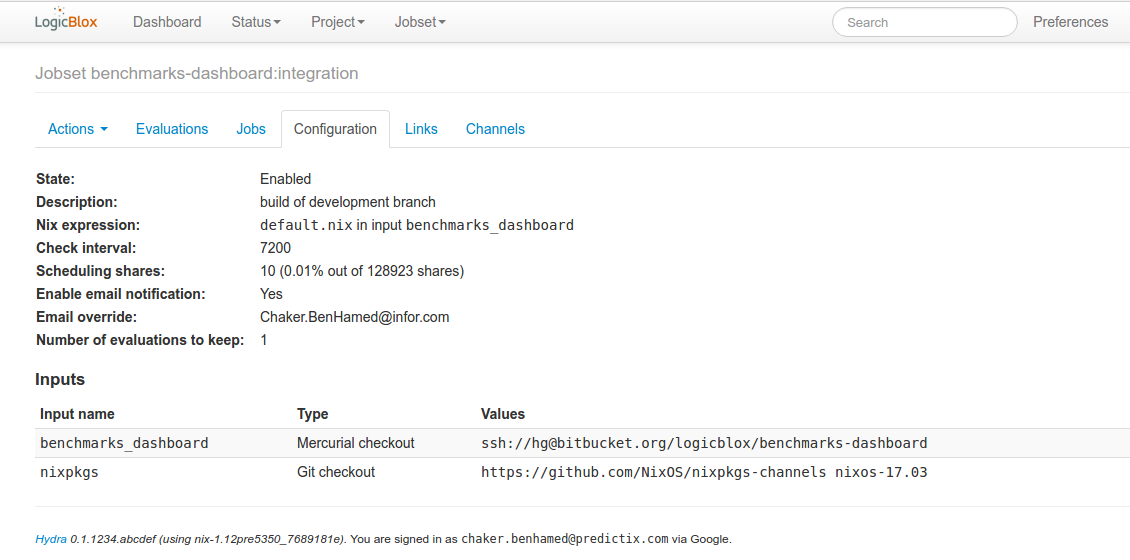
\includegraphics[width=17cm]{hydra_configuration}
\caption{Benchmarks Dashboard Hydra configuration screen}
\label{fig:hydra_configuration}
\end{figure}

The figure \hyperref[fig:hydra_eval]{\ref{fig:hydra_eval}} represents the Hydra
evaluation screen, where we can see the history if the build and whether there
are erros in the build or not.

\begin{figure}[h]
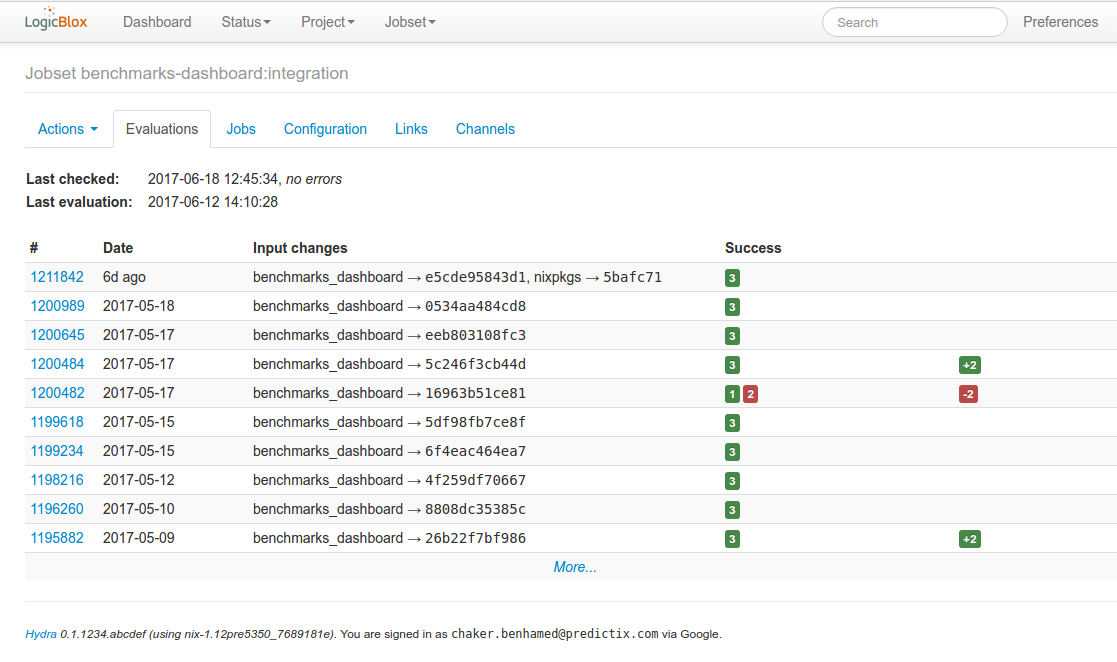
\includegraphics[width=17cm]{hydra_eval}
\caption{Benchmarks Dashboard Hydra configuration screen}
\label{fig:hydra_eval}
\end{figure}

In Hydra we can also run unit test and report various indicator about the
quality of the application. The figure
\hyperref[fig:coverage]{\ref{fig:coverage}} shows the covarge report of the test
of our application.

\begin{figure}[h]
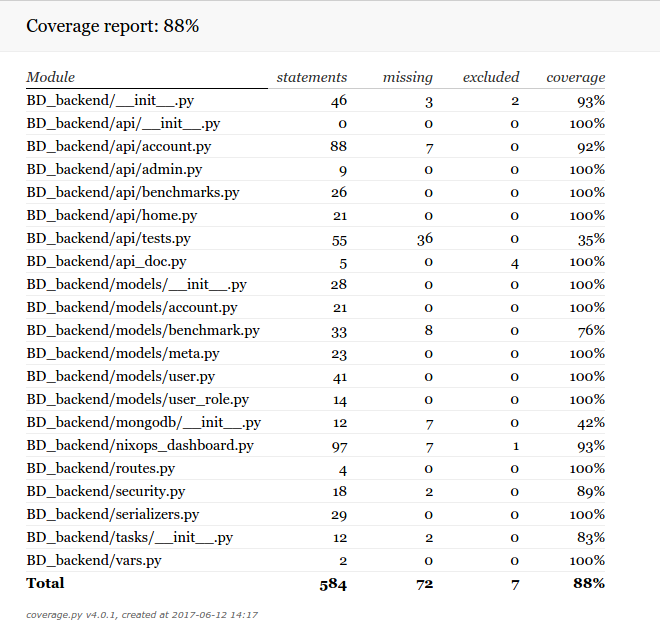
\includegraphics[width=17cm]{coverage}
\caption{Coverage report}
\label{fig:coverage}
\end{figure}

\section*{Conclusion}
TODO
